\documentclass[10pt,portrait]{article}
\usepackage[]{mathpazo}
\usepackage{amssymb,amsmath}
\usepackage{ifxetex,ifluatex}
\usepackage{fixltx2e} % provides \textsubscript
\ifnum 0\ifxetex 1\fi\ifluatex 1\fi=0 % if pdftex
  \usepackage[T1]{fontenc}
  \usepackage[utf8]{inputenc}
\else % if luatex or xelatex
  \ifxetex
    \usepackage{mathspec}
  \else
    \usepackage{fontspec}
  \fi
  \defaultfontfeatures{Ligatures=TeX,Scale=MatchLowercase}
\fi
% use upquote if available, for straight quotes in verbatim environments
\IfFileExists{upquote.sty}{\usepackage{upquote}}{}
% use microtype if available
\IfFileExists{microtype.sty}{%
\usepackage{microtype}
\UseMicrotypeSet[protrusion]{basicmath} % disable protrusion for tt fonts
}{}
\usepackage[margin=3mm]{geometry}
\usepackage{hyperref}
\hypersetup{unicode=true,
            pdftitle={Note of STAT 671},
            pdfborder={0 0 0},
            breaklinks=true}
\urlstyle{same}  % don't use monospace font for urls
\usepackage{graphicx,grffile}
\makeatletter
\def\maxwidth{\ifdim\Gin@nat@width>\linewidth\linewidth\else\Gin@nat@width\fi}
\def\maxheight{\ifdim\Gin@nat@height>\textheight\textheight\else\Gin@nat@height\fi}
\makeatother
% Scale images if necessary, so that they will not overflow the page
% margins by default, and it is still possible to overwrite the defaults
% using explicit options in \includegraphics[width, height, ...]{}
\setkeys{Gin}{width=\maxwidth,height=\maxheight,keepaspectratio}
\IfFileExists{parskip.sty}{%
\usepackage{parskip}
}{% else
\setlength{\parindent}{0pt}
\setlength{\parskip}{6pt plus 2pt minus 1pt}
}
\setlength{\emergencystretch}{3em}  % prevent overfull lines
\providecommand{\tightlist}{%
  \setlength{\itemsep}{0pt}\setlength{\parskip}{0pt}}
\setcounter{secnumdepth}{5}
% Redefines (sub)paragraphs to behave more like sections
\ifx\paragraph\undefined\else
\let\oldparagraph\paragraph
\renewcommand{\paragraph}[1]{\oldparagraph{#1}\mbox{}}
\fi
\ifx\subparagraph\undefined\else
\let\oldsubparagraph\subparagraph
\renewcommand{\subparagraph}[1]{\oldsubparagraph{#1}\mbox{}}
\fi

%%% Use protect on footnotes to avoid problems with footnotes in titles
\let\rmarkdownfootnote\footnote%
\def\footnote{\protect\rmarkdownfootnote}

%%% Change title format to be more compact
\usepackage{titling}

% Create subtitle command for use in maketitle
\providecommand{\subtitle}[1]{
  \posttitle{
    \begin{center}\large#1\end{center}
    }
}

\setlength{\droptitle}{-2em}

  \title{Note of STAT 671}
    \pretitle{\vspace{\droptitle}\centering\huge}
  \posttitle{\par}
  \subtitle{Statistical Learning I 2019}
  \author{}
    \preauthor{}\postauthor{}
    \date{}
    \predate{}\postdate{}
  
\usepackage{multicol}
\usepackage{multirow}
\usepackage{caption}
\setlength\tabcolsep{0.1pt}
\setlength\lineskip{0pt}
\setlength\parskip{0pt}

\begin{document}
\maketitle

{
\setcounter{tocdepth}{4}
\tableofcontents
}
\hypertarget{section}{%
\section{}\label{section}}

\hypertarget{kernel-1002}{%
\subsection{\texorpdfstring{Kernel
\texttt{10/02}}{Kernel 10/02}}\label{kernel-1002}}

\begin{itemize}
\tightlist
\item
  Cat and Dog problem
\end{itemize}

\hypertarget{a-simple-geometric-solution}{%
\subsubsection{A simple geometric
solution}\label{a-simple-geometric-solution}}

\begin{itemize}
\tightlist
\item
  \(\mathcal{X}\mapsto\mathbb{R}^2\), Training set:
\end{itemize}

\[T=\{(x_i,y_i);x_i\in\mathcal{X},y_i\in\{-1;+1\}\}\]

Notate \(I_+=\{i;y_i=+1\},\ I_-=\{i;y_i=-1\}\) Number of
\(I_+=n_+;\ I_-=n_-;\ T=n=n_++n_-\)

\[C_+=\frac1{n_{+}}\sum\limits_{i\in I_+}^n x_i;\quad C_-=\frac1{n_{-}}\sum\limits_{i\in I_-}^n x_i;\quad C=\frac1{2}(C_++C_-)\]

\begin{itemize}
\tightlist
\item
  Deifne the generalized ``simple classifier''
  \(g: \mathbb{R}^2\to\mathbb{R}\)
\end{itemize}

\begin{eqnarray*}
g(x)&=\langle C_+-C_-,X-C\rangle_{\mathbb{R}^2}=(X-C)^T(C_+-C_-)\\
    &=\langle X,C_+\rangle-\langle X,C_-\rangle+b
\end{eqnarray*}

\begin{itemize}
\tightlist
\item
  A binary ``simple classifier'' is then
  \(f(x)=\begin{cases}+1&\text{if }g(x)\ge0\\-1&\text{if }g(x)<0\end{cases}\)
\end{itemize}

Let us write \(g(x)\) using
\(\langle \cdot,\cdot\rangle_{\mathbb{R}^2}\) such that we can propose
other classifiers by using the kernel trick, that is reproduing
\(\langle \cdot,\cdot\rangle_{\mathbb{R}^2}\) by \(k(\cdot,\cdot)\) a
p.d. kernel.

\[g(x)=\langle C_+,X\rangle -\langle C_-,X\rangle -\langle C_+,C\rangle +\langle C_-,C\rangle\]

\(\langle C_+,X\rangle =\frac1{n_{+}}\sum\limits_{i\in I_+}^n\langle x_i,x\rangle\);

\(\langle C_-,X\rangle =\frac1{n_{-}}\sum\limits_{i\in I_-}^n\langle x_i,x\rangle\);

\(\langle C_+,C\rangle =\langle C_+,\frac12C_+\rangle +\langle C_+,\frac12C_-\rangle =\frac1{2n_{+}^2}\sum\limits_{(i,j)\in I_{+}}\langle x_i,x_j\rangle +\frac12\langle C_+,C_-\rangle\)

\(\langle C_-,C\rangle =\langle C_-,\frac12C_+\rangle +\langle C_-,\frac12C_-\rangle =\frac12\langle C_+,C_-\rangle +\frac1{2n_{-}^2}\sum\limits_{(i,j)\in I_{-}}\langle x_i,x_j\rangle\)

\[g(x)=\frac1{n_{+}}\sum\limits_{i\in I_+}^n\langle x_i,x\rangle-\frac1{n_{-}}\sum\limits_{i\in I_-}^n\langle x_i,x\rangle -\frac1{2n_{+}^2}\sum\limits_{(i,j)\in I_{+}}\langle x_i,x_j\rangle-\frac12\langle C_+,C_-\rangle +\frac12\langle C_+,C_-\rangle +\frac1{2n_{-}^2}\sum\limits_{(i,j)\in I_{-}}\langle x_i,x_j\rangle\]

\[=\sum_{i=1}^n\alpha_i\langle x_i,x\rangle +b;
\text{where } \alpha_i=\begin{cases}\frac1{n_{+}}&y_i=+1\\\frac{-1}{n_{-}}&y_i=-1\end{cases};\ b=\frac1{2n_{-}^2}\sum\limits_{(i,j)\in I_{-}}\langle x_i,x_j\rangle -\frac1{2n_{+}^2}\sum\limits_{(i,j)\in I_{+}}\langle x_i,x_j\rangle\]

\hypertarget{a-more-general-solution}{%
\subsubsection{A more general solution}\label{a-more-general-solution}}

We notice that in this cunstruction, the mapping \(x\mapsto\mathcal{H}\)
appears only through
\(k(x,x')=\langle\phi(x),\phi(x')\rangle_{\mathcal{H}}\)

k is a positive definite kernel. \(\mathcal{H}\) and \(\phi\) such that
\(k(x,x')=\langle\phi(x),\phi(x')\rangle_{\mathcal{H}}\) .

For any \(x,x'\in\mathcal{X}\neq\phi\), \(\phi: x \mapsto \mathcal{H}\),
\(k(x,x')=\langle\phi(x),\phi(x')\rangle_{\mathcal{H}}\)

\begin{itemize}
\item
  Properties of k
\item
  Symmetric \(k(x,x')=k(x',x)\)
\item
  positive \(\|\sum_{i=1}^n\alpha_i\phi(x_i)\|_{\mathcal{H}}^2\ge0\)
\end{itemize}

\(\langle\sum_{i=1}^n\alpha_i\phi(x_i),\sum_{j=1}^n\alpha_j\phi(x_j)\rangle_{\mathcal{H}}=\sum_{i=1}^n\sum_{j=1}^n\alpha_i\alpha_j\langle\phi(x_i),\phi(x_j)\rangle_{\mathcal{H}}\)

K is a positive definite kernel, \(\mathcal{H}\) is a Hilbert Space of
function \(\mathcal{X}\mapsto\mathbb{R}\).

\hypertarget{polynomial-kernel-1007}{%
\subsection{\texorpdfstring{Polynomial Kernel
\texttt{10/07}}{Polynomial Kernel 10/07}}\label{polynomial-kernel-1007}}

\(x\in\mathbb{R}^2, x=(x_1,x_2)^T\)

\hypertarget{example-0-linear-kernel}{%
\subsubsection{Example 0: Linear kernel}\label{example-0-linear-kernel}}

\(k(x,x')=\langle x,x'\rangle_\mathbb{R^2}=x^Tx'=x_1x'_1+x_2x'_2\)

Chech that this kernel is p.d.

Let \(\phi=I,H=\mathbb{R^2}\), Find
\(k(x,x')=\langle\phi(x),\phi(x')\rangle_{\mathcal{H}}\)

\(\sum_{i=1}^n\sum_{j=1}^n\alpha_i\alpha_jk(x_i,x_j)=\alpha^Tx^Tx\alpha=\|\alpha x\|^2\ge0\)

\hypertarget{example-1-phi-mathbbr4tomathbbr2}{%
\subsubsection{\texorpdfstring{Example 1
\(\phi: \mathbb{R}^4\to\mathbb{R}^{2}\)}{Example 1 \textbackslash{}phi: \textbackslash{}mathbb\{R\}\^{}4\textbackslash{}to\textbackslash{}mathbb\{R\}\^{}\{2\}}}\label{example-1-phi-mathbbr4tomathbbr2}}

\(x=(x_1,x_2) \in \mathbb{R}^2\),
\(\phi(x)=(x_1^2,x_1x_2,x_2x_1,x_2^2)^T\)

\(k(x,y)=\langle\phi(x),\phi(y)\rangle_{\mathbb{R^4}}=x_1^2y_1^2+2x_1x_2y_1y_2+x_2^2y_2^2=\langle x_1,y_1\rangle^2_{\mathbb{R^2}}+2\langle x_1,y_1\rangle\langle x_2,y_2\rangle+\langle x_2,y_2\rangle^2_{\mathbb{R^2}}\)

\(\phi: \mathbb{R}^2\to\mathbb{R}^{2^3}\)

\(\phi(x)=(x_1^3, x_1^2x_2, x_2x_1^2, x_1x_2x_1, x_2x_1x_2, x_1x_2^2, x_2^2x_1, x_2^3)^T\)

\(k(x,y)=\langle\phi(x),\phi(y)\rangle_{\mathbb{R^8}}=x_1^3y_1^3+3x_1^2x_2y_1^2y_2+3x_1x_2^2y_1y_2^2+x_2^3y_2^3=\langle x,y\rangle^3_{\mathbb{R^2}}=(x_1y_1+x_2y_2)^3\)

\hypertarget{example-2-mathcalxmathbbrn}{%
\subsubsection{\texorpdfstring{Example 2
\(\mathcal{X}=\mathbb{R}^n\)}{Example 2 \textbackslash{}mathcal\{X\}=\textbackslash{}mathbb\{R\}\^{}n}}\label{example-2-mathcalxmathbbrn}}

\(\phi(x)=\{x_{j1},..,x_{jd};1\le j1,..jd\le n\}\), \(n^d\) iterms

\(k(x,y)=\langle\phi(x),\phi(y)\rangle_{\mathbb{R^{n^d}}}=\langle x,y\rangle^d_{\mathbb{R^n}}\)

\hypertarget{cauchy-schwarts-inequity-for-kernels}{%
\subsubsection{Cauchy-Schwarts inequity for
kernels}\label{cauchy-schwarts-inequity-for-kernels}}

\(x,x'\in\mathcal{X}\neq\phi\),
\(k: \mathcal{X}\times\mathcal{X} \to \mathbb{R}\) is a positive
definite kernel, proposition for any \(x,x'\)

\[k^2(x,x')\le k(x,x)k(x',x')\]

Proof: \(n=2, x=(x_1,x_2), \alpha=(\alpha_1, \alpha_2)\)

\(\sum_{i=1}^n\sum_{j=1}^n\alpha_i\alpha_jk(x_i,x_j)\ge0 \iff\) the Gram
matrix
\(\begin{pmatrix}k(x_1,x_1)&k(x_1,x_2)\\k(x_2,x_1)&k(x_2,x_2)\end{pmatrix}\)
semi-positive definite or equvalent determinant \(\ge0\)

\[k(x_1,x_1)k(x_2,x_2)- k(x_1,x_2)k(x_2,x_1)\ge0\implies k(x_1,x_1)k(x_2,x_2)\ge k^2(x_1,x_2)\]

\hypertarget{rkhs-1009}{%
\subsection{\texorpdfstring{RKHS
\texttt{10/09}}{RKHS 10/09}}\label{rkhs-1009}}

Reproducing Kernel Hilbert Space

A Hilbert Space is a complete inner product space.

A inner product space is a vector space with an inner product (dot
product, scalar product).

Dot product \(\vec a\vec b=a_xb_x+a_yb_y=|\vec a||\vec b|\cos(\theta)\)

Start with a vector space (H,+,\(\cdot\)) over \(\mathbb{R}\) (\(\cdot\)
scalor multiplication)

An inner product is a mapping: \(H\times H\to\mathbb{R}\) such that

\begin{enumerate}
\def\labelenumi{\arabic{enumi}.}
\item
  \(\langle f,g\rangle=\langle g,f\rangle\) symmetry for any
  \(f,g\in H\)
\item
  \(\langle\alpha f_1+\beta f_2,g\rangle=\alpha\langle f_1,g\rangle+\beta\langle f_2,g\rangle\)
  for any \(f,g\in H;\alpha,\beta\in\mathbb{R}\)
\item
  \(\langle f,f\rangle\ge0\) for all \(f\in H\)
\item
  \(\langle f,f\rangle=0\iff f=0_H\)
\end{enumerate}

We can define \(\|f\|^2=\langle f,f\rangle\) that defines a Norm on
\(H\)

A metric space is complete for an inner product when it cantains the
limit fo all the Cauchy sequences for this inner product.

\begin{itemize}
\item
\end{itemize}

\(x,x'\in\mathcal{X}\neq\phi\), \(\phi\in\mathcal{H}\)

K is a positive definite kernel, \(\mathcal{H}\) is a Hilbert Space of
function \(\mathcal{X}\mapsto\mathbb{R}\).

We known that if a function
\(k: \mathcal{X}\times\mathcal{X}\mapsto\mathbb{R}\) verifies
\(k(x,x')=\langle\phi(x),\phi(x')_{\mathcal{H}}\), then it is a positive
kernel

\begin{itemize}
\tightlist
\item
  Reverse: Aronsjar Theorem
\end{itemize}

If k is a positive definite kernel then there exist \(\mathcal{H}\) and
\(\phi\) such that \(k(x,x')=\langle\phi(x),\phi(x')_{\mathcal{H}}\) is
true.

Let us start with k and come up with \(\mathcal{H}\) and \(\phi\) :
\(\mathcal{X}, k(\cdot,\cdot)\)

Let us start \(\mathcal{H}\) with the function \(k(\cdot,x)\) for all
\(x\in\mathcal{X}\)

\hypertarget{example-0-linear-kernel-1}{%
\subsubsection{Example 0: Linear
kernel}\label{example-0-linear-kernel-1}}

\(\mathcal{X}=\mathbb{R}, k(x,x')=xx'\), \(k(\cdot,x): y\mapsto yx\)

\hypertarget{example-1-gaussian-kernel-with-parametor-sigma2}{%
\subsubsection{\texorpdfstring{Example 1: Gaussian kernel with parametor
\(\sigma^2\)}{Example 1: Gaussian kernel with parametor \textbackslash{}sigma\^{}2}}\label{example-1-gaussian-kernel-with-parametor-sigma2}}

\(k(\cdot,x): y\mapsto \exp[-\frac1{2\sigma^2}(y-x)^2]\)

Let us create a vector space by adding all the finite linear combination
of \(k(\cdot,x),x\in\mathcal{X}\)

\[V=\{f:\mathcal{X}\to\mathbb{R},\ f(x)=\sum_{i=1}^n\alpha_ik(x,x_i)\ \text{  for some  } n\ge1;\ x_1,..,x_n\in\mathcal{X};\alpha_1,..,\alpha_n\in\mathbb{R}\}\]

\[f\in V\leftrightarrow\begin{Bmatrix}\ x_1,..,x_n\\\alpha_1,..,\alpha_n\end{Bmatrix}\quad 
  g\in V\leftrightarrow\begin{Bmatrix}\ y_1,..,y_m\\\beta_1,..,\beta_m\end{Bmatrix}\quad 
  f+g\leftrightarrow\begin{Bmatrix}\ x_1,..,x_n,y_1,..,y_m\\\alpha_1,..,\alpha_n,\beta_1,..,\beta_m\end{Bmatrix}\quad 
  \gamma f\leftrightarrow\begin{Bmatrix}\ x_1,..,x_n\\\gamma\alpha_1,..,\gamma\alpha_n\end{Bmatrix},\gamma\in\mathbb{R}\]

\[\gamma_1f+\gamma_2g\leftrightarrow\begin{Bmatrix}\ \overbrace{x_1,..,x_n}^{z_1,..,z_n},\overbrace{y_1,..,y_m}^{z_{n+1},..,z_{n+m}}\\
                     \underbrace{\gamma_1\alpha_1,..,\gamma_1\alpha_n}_{\delta_1,..,\delta_n},\underbrace{\gamma_2\beta_1,..,\gamma_2\beta_m}_{\delta_{n+1},..,\delta_{n+m}}\end{Bmatrix}
                     \leftrightarrow h(x)=\sum_{i=1}^{n+m}\delta_ik(x,z_i)\]

\[(\gamma_1f+\gamma_2g)(x)=\gamma_1\sum_{i=1}^n\alpha_ik(x,x_i)+\gamma_2\sum_{i=1}^m\beta_ik(x,y_i)=\gamma_1f(x)+\gamma_2g(x)\]

Note: the representation
\(\begin{Bmatrix}\ x_1,..,x_n\\\alpha_1,..,\alpha_n\end{Bmatrix}\) of a
function in V is not necessary unique

\begin{itemize}
\tightlist
\item
  Define
  \(\langle f,g\rangle=\sum_{i=1}^n\alpha_i\sum_{j=1}^m\beta_ik(x_i,y_j)\)
  is a function \(\mathcal{X}\times\mathcal{X}\mapsto\mathbb{R}\)
\end{itemize}

\(f\in V\leftrightarrow\begin{Bmatrix}\ x_1,..,x_n\\\alpha_1,..,\alpha_n\end{Bmatrix};g\in V\leftrightarrow\begin{Bmatrix}\ y_1,..,y_m\\\beta_1,..,\beta_m\end{Bmatrix}\)

\[\langle f,g\rangle=\sum_{i=1}^n\alpha_i\underbrace{\sum_{j=1}^m\beta_ik(x_i,y_j)}_{g(x_i)}=\sum_{i=1}^n\alpha_ig(x_i)
=\sum_{j=1}^m\beta_i\underbrace{\sum_{i=1}^n\alpha_ik(y_j,x_i)}_{f(y_j)}=\sum_{j=1}^m\beta_if(y_j)\]

which shows that \(\langle f,g\rangle\) does not depend on the
particular representation of \((f,g)\)

So it is a function \(\mathcal{X}\times\mathcal{X}\mapsto\mathbb{R}\)

\(\langle f,k(\cdot,x)\rangle=\sum_{i=1}^n\alpha_ik(x_i,x)=f(x)\)

\(\langle k(\cdot,y),k(\cdot,x)\rangle=k(x,y)\)

\hypertarget{rkhs-construction-and-definitions-1014}{%
\subsection{\texorpdfstring{RKHS construction and definitions
\texttt{10/14}}{RKHS construction and definitions 10/14}}\label{rkhs-construction-and-definitions-1014}}

, \(\phi\in\mathcal{H}\)

K is a positive definite kernel over \(\mathcal{X}\neq\phi\) \(\iff\)
There is some Hilbert Space \(\mathcal{H}\) and some mapping
\(\phi: x\mapsto\mathcal{H}\) such that
\(k(x,y)=\langle\phi(x),\phi(y)\rangle_{\mathcal{H}}\) is true for every
\((x,y)\in \mathcal{X}\times\mathcal{X}\)

For constructing \(t\mapsto k(t,x), x\in\mathbb{R}\), add linear
combinations

\[f:\mathcal{X}\mapsto\mathbb{R};\ f(x)=\sum_{i=1}^n\alpha_ik(x,x_i);\ g(x)=\sum_{j=1}^m\beta_jk(x,y_j)\]

\begin{itemize}
\tightlist
\item
  Define
  \(\langle f,g\rangle=\sum_{i=1}^n\sum_{j=1}^m\alpha_i\beta_ik(x_i,y_j)\)
\end{itemize}

\begin{enumerate}
\def\labelenumi{\arabic{enumi}.}
\item
  not depend on the ``represenation'' in term of
  \(\begin{Bmatrix}\ x_1,..,x_n\\\alpha_1,..,\alpha_n\end{Bmatrix}; \begin{Bmatrix}\ y_1,..,y_m\\\beta_1,..,\beta_m\end{Bmatrix}\)
\item
  \(\langle f,g\rangle=\langle g,f\rangle\)
\item
  Linearity
  \(\langle f+g,h\rangle=\langle f,h\rangle+\langle g,h\rangle;\ \alpha\langle f,g\rangle=\alpha\langle f,g\rangle\)
\item
  \(\langle f,f\rangle\ge0\iff\) k has the definite positive property
\end{enumerate}

\(\langle f,k(\cdot,x)\rangle=\sum_{i=1}^n\alpha_ik(x_i,x)=f(x)\),
\(f\in\begin{Bmatrix}\ x_1,..,x_n\\\alpha_1,..,\alpha_n\end{Bmatrix}\);
\(k(\cdot,x)=(x,1)^T\)

\(k(x,y)=\langle\phi(x),\phi(y)\rangle=\langle k(\cdot,y),k(\cdot,x)\rangle=\langle k(\cdot,x),k(\cdot,y)\rangle\)

\begin{itemize}
\tightlist
\item
  Proof \(\langle f,f\rangle=0\implies f=0\iff\) for any
  \(x\in\mathcal{X}, f(x)=0\)
\end{itemize}

Step 1 check that \(\langle f,g\rangle\) is p.d.;

\(f_1,..f_n\), scalar \(\gamma_1,..,\gamma_n\)

\[\sum_{i=1}^n\sum_{j=1}^n\gamma_i\gamma_j\langle f_i,f_j\rangle=\langle\sum_{i=1}^n\gamma_i f_i,\sum_{j=1}^n\gamma_jf_j\rangle\ge0, g\in H\]

Step 2 Use Cauchy-Schwarz inequality for \(\langle f,g\rangle\)

\(x\in\mathcal{X},f\in\mathcal{H}\)

\[|f(x)|^2=|\langle f,k(\cdot,x)\rangle|^2\le\|f\|^2\|k(\cdot,x)\|^2=\|f\|^2k(x,x)\]
then for any \(x\in\mathcal{X}\),
\(\|f\|^2=\langle f,f\rangle=0\implies|f(x)|^2=0\implies f(x)=0\)

We have shown that (\(H,\langle\cdot,\cdot\rangle\)) just constructed to
a inner product space pre-Hilbert Space.

It can be completed into a Hilbert Space by including the limits of
convergent Cauchy sequances

\begin{itemize}
\tightlist
\item
  Define RKHS 1
\end{itemize}

\(X\neq\phi\), \(\mathcal{H}\) is a Hilbert Space of function
\(\mathcal{X}\mapsto\mathbb{R}\)

\(\mathcal{H}\) is a Reproducing Kernel Hilbert Space when there is a
function \(k: \mathcal{X}\times\mathcal{X}\mapsto\mathbb{R}\) such that

\begin{enumerate}
\def\labelenumi{\arabic{enumi}.}
\item
  \(k(\cdot,x)\in{\mathcal{H}}\) for all \(x\in\mathcal{X}\)
\item
  Reproducing Property
  \(\langle\underbrace{ f}_{function},\underbrace{k(\cdot,x)}_{argument}\rangle_{\mathcal{H}}=f(x)\)
  for any \(f\in\mathcal{H}\)
\end{enumerate}

\hypertarget{example-0-mathcalxinmathbbrdquad-kxyxty}{%
\subsubsection{\texorpdfstring{Example 0:
\(\mathcal{X}\in\mathbb{R}^d,\quad k(x,y)=x^Ty\)}{Example 0: \textbackslash{}mathcal\{X\}\textbackslash{}in\textbackslash{}mathbb\{R\}\^{}d,\textbackslash{}quad k(x,y)=x\^{}Ty}}\label{example-0-mathcalxinmathbbrdquad-kxyxty}}

The RKHS with kernel k is

\[\mathcal{H} = \{f_w:\ \mathbb{R}^d\mapsto\mathbb{R};\ f_w(x)=w^Tx;\quad w\in\mathbb{R}^d\}\]

\[\langle f_v,f_w\rangle_{\mathcal{H}}=v^Tw\implies\langle f_v,f_v\rangle=\|f_v\|^2_{\mathcal{H}}=\|v\|^2\]
Let us check that \(\mathcal{H}\) is the RKHS associated with k

\(t\mapsto k(t,x)=x^Tt=(x^Tt)^T=t^Tx=f_t(x)\)

Exercise:

\(\langle f,k(\cdot,x)\rangle=\langle f_w,f_x\rangle=x^Tw=(x^Tw)^T=w^Tx=f_w(x)\)

\hypertarget{example-1-mathcalxinmathbbrdquad-kxyxtycc0}{%
\subsubsection{\texorpdfstring{Example 1:
\(\mathcal{X}\in\mathbb{R}^d,\quad k(x,y)=x^Ty+c,c>0\)}{Example 1: \textbackslash{}mathcal\{X\}\textbackslash{}in\textbackslash{}mathbb\{R\}\^{}d,\textbackslash{}quad k(x,y)=x\^{}Ty+c,c\textgreater{}0}}\label{example-1-mathcalxinmathbbrdquad-kxyxtycc0}}

\[\mathcal{H} = \{f:\ \mathbb{R}^d\mapsto\mathbb{R};\ f_{w,w_0}(x)=w^Tx+w_0;\quad w\in\mathbb{R}^d,w_0\in\mathbb{R}\}\]
\[\langle f_{v,v_0},f_{w,w_0}\rangle_{\mathcal{H}}=v^Tw+\frac1cv_0w_0\implies\langle f_{v,v_0},f_{v,v_0}\rangle=\|f_{v,v_0}\|^2_{\mathcal{H}}=\|v\|^2+\frac{v_0^2}c\]
What is the RKHS associated with \(k_c\)?

\(t\mapsto k(t,x)=x^Tt=(x^Tt)^T=t^Tx=f_t(x)\)

\[\langle f_{w,w_0},k(\cdot,x)\rangle=\langle f_{w,w_0},f_x\rangle=x^Tw+\frac1cxw_0=(x^Tw+c)^T+w_0=w^Tx+w_0=f_w(x)\]

\begin{itemize}
\tightlist
\item
  Define RKHS 2
\end{itemize}

\(X\neq\phi\), \(\mathcal{H}\) is a Hilbert Space of function
\(\mathcal{X}\mapsto\mathbb{R}\)

\(\mathcal{H}\) is a RKHS if and only if for any \(f\in{\mathcal{H}}\),
\(x\in\mathcal{X}\)

the evaluation function \(\mathcal{H}\mapsto\mathbb{R}\):
\(F_x: f\mapsto f(x)\) is continuous

\(f,g\in\mathcal{H}\) if \(\|f-g\|\) is small then their different
\(|f(x)-g(x)|\) is small.

\hypertarget{two-definitions-of-rkhs-why-equvalent-1016}{%
\subsection{\texorpdfstring{Two Definitions of RKHS (why equvalent)
\texttt{10/16}}{Two Definitions of RKHS (why equvalent) 10/16}}\label{two-definitions-of-rkhs-why-equvalent-1016}}

\(X\neq\phi\), \(\mathcal{H}\): Hilbert Space of function
\(\mathcal{X}\mapsto\mathbb{R}\)

Example: \(\mathcal{X}=\{x_1,..x_n\}\);
\(\begin{bmatrix} f(x_1)\\\vdots\\f(x_n) \end{bmatrix}\subset\{\text{vector of}\ \mathbb{R}^n\}\)

\hypertarget{definition-1}{%
\subsubsection{Definition 1:}\label{definition-1}}

\(\mathcal{H}\) is a RKHS when there is a function
\(\mathcal{X}\times\mathcal{X}\mapsto\mathbb{R}\), \(K(\cdot,\cdot)\)
such that

\begin{itemize}
\item
  A: \(t\mapsto k(t,x)\in\mathcal{H}\) for each \(x\)
\item
  B: \(\langle f,k(\cdot,x)\rangle_{\mathcal{H}}=f(x)\) for each
  \(f\in\mathcal{H}\), \(x\in\mathcal{X}\)

  -- Reproducing Property
\end{itemize}

\hypertarget{definition-2}{%
\subsubsection{Definition 2:}\label{definition-2}}

\(\mathcal{H}\) is a RKHS when the evaluation functions

\begin{eqnarray*}
F_x: & \mathcal{H}&\mapsto\mathbb{R} \\& f&\mapsto f(x) \quad \text{are continuous.}
\end{eqnarray*}

\hypertarget{definition-1-implies-definition-2}{%
\subsubsection{\texorpdfstring{Definition 1 \(\implies\) Definition
2}{Definition 1 \textbackslash{}implies Definition 2}}\label{definition-1-implies-definition-2}}

\(F_x\) is continuous. if

\begin{eqnarray*}
&\|f-g\|_{\mathcal{H}}&<\delta \quad\text{(might depend on x)}\\ \implies &|f(x)-g(x)| & <  \varepsilon
\end{eqnarray*}

\(F_x\) is \emph{C-Lipschitz} continuous when
\[|f(x)-g(x)|  \le  c\|f-g\|_{\mathcal{H}},\quad c>0, \quad\text{for any}\ f,\ g\in\mathcal{H}\]
\emph{C-Lipschitz} \(\implies\) continuity.

\[|f(x)-g(x)|=|(f-g)(x)|=|\langle f-g,k(\cdot,x)\rangle_{\mathcal{H}}|\le  \|f-g\|_{\mathcal{H}}\ \underbrace{\langle k(\cdot,x),k(\cdot,x)\rangle^{\frac12}}_{k^{\frac12}(x,x)}\]

\hypertarget{definition-2-implies-definition-1}{%
\subsubsection{\texorpdfstring{Definition 2 \(\implies\) Definition
1}{Definition 2 \textbackslash{}implies Definition 1}}\label{definition-2-implies-definition-1}}

\begin{quote}
\emph{Riesz Representation Theorem}: In any Hilber Space of function
\(\mathcal{X}\mapsto\mathbb{R}\) for which \(F_x\) is continuous for
each \(x\in\mathcal{X}\), then there is an unique element of
\(\mathcal{H}\), notated \(g_x\), for which
\(f(x)=\langle f,g_x\rangle_\mathcal{H}\) for each
\(f\in\mathcal{H},\quad g_x(\cdot)=k(\cdot,x)\).
\end{quote}

\hypertarget{examples}{%
\subsection{Examples}\label{examples}}

\hypertarget{example-0-mathcalxinmathbbrdquad-kxyxty-1}{%
\subsubsection{\texorpdfstring{Example 0:
\(\mathcal{X}\in\mathbb{R}^d,\quad k(x,y)=x^Ty\)}{Example 0: \textbackslash{}mathcal\{X\}\textbackslash{}in\textbackslash{}mathbb\{R\}\^{}d,\textbackslash{}quad k(x,y)=x\^{}Ty}}\label{example-0-mathcalxinmathbbrdquad-kxyxty-1}}

\hypertarget{example-1-mathcalxx_1..x_n}{%
\subsubsection{\texorpdfstring{Example 1:
\(\mathcal{X}=\{x_1,..x_n\}\),}{Example 1: \textbackslash{}mathcal\{X\}=\textbackslash{}\{x\_1,..x\_n\textbackslash{}\},}}\label{example-1-mathcalxx_1..x_n}}

notate \(\underset{{(n,n)}}{k}\); \({[k]}_{ij}=k(x_i,x_j)\). \(k\) is
symmetric and positive semi-definite.

Assume that \(k\) is positive definite,

\[f:\ \mathcal{X}\mapsto\mathbb{R},\quad  \begin{bmatrix} f(x_1)\\\vdots\\f(x_n) \end{bmatrix}\subset\ \mathbb{R}^n\]

\[k(\cdot,x_i)=\begin{bmatrix} k_{1i}\\\vdots\\k_{ni} \end{bmatrix}=k_i\ ;\quad k=(k_1,..k_n)\]

\begin{eqnarray*}
\mathcal{H}  &= & \{ \alpha_1k_1+\cdots+\alpha_nk_n;\ \alpha_1,\cdots,\alpha_n\in\mathbb{R}\} \\ & = & \text{Span}\{k_1,..k_n\}=\mathbb{R}^n \quad \text{is a vector space.}
\end{eqnarray*}

\begin{eqnarray*}
\langle f,g\rangle_{\mathcal{H}}&=&f^Tk^{-1}g\\ \langle f,k(\cdot,x_i)\rangle &=& \langle f,ke_i \rangle,\quad e_i=\begin{bmatrix} 0\\\vdots \\1 \\\vdots\\0 \end{bmatrix}\begin{matrix} \\ \\\leftarrow i \\ \\ \\ \end{matrix}\\
&=&f^T\underbrace{k^{-1}k}_{I}e_i\\
&=&f^Te_i\\
&=&\begin{bmatrix} f(x_1)&\hdots&f(x_n) \end{bmatrix}\begin{bmatrix} 0\\\vdots \\1 \\\vdots\\0 \end{bmatrix}\begin{matrix} \\ \\\leftarrow i \\ \\ \\ \end{matrix}\\
&=&f(x_i)
\end{eqnarray*}

\hypertarget{example-2-mathcalxinmathbbrnquad-kxyxty2}{%
\subsubsection{\texorpdfstring{Example 2:
\(\mathcal{X}\in\mathbb{R}^n,\quad k(x,y)=(x^Ty)^2\)}{Example 2: \textbackslash{}mathcal\{X\}\textbackslash{}in\textbackslash{}mathbb\{R\}\^{}n,\textbackslash{}quad k(x,y)=(x\^{}Ty)\^{}2}}\label{example-2-mathcalxinmathbbrnquad-kxyxty2}}

\[\mathcal{H} = \{f:\ f(x)=x^TS_x;\quad \underset{{(n,n)}}{S}\ \text{is a symmetric Matrix}\}\]
verify this is a Hilbert Space.

\[\langle f_{S_1},f_{S_2}\rangle_{\mathcal{H}}=\langle S_1,S_2\rangle_{\mathcal{F}}=\sum\limits_{i,j=1}^n[S_1]_{ij}[S_2]_{ij}\]

\[ \langle f_{S_1},k(\cdot,x_i)\rangle = f_{S_1}(x)\quad \text{check it}\]

\[k(y,x)=(y^Tx)(y^Tx)=y^T\cdot \underbrace{xx^T}_{\substack{(n,n)\\ \text{symmetric}\\ \text{matrix}}}\cdot y\]

\begin{document}
\raggedright
\footnotesize
\begin{multicols}{3}


% multicol parameters
% These lengths are set only within the two main columns
%\setlength{\columnseprule}{0.25pt}
\setlength{\premulticols}{1pt}
\setlength{\postmulticols}{1pt}
\setlength{\multicolsep}{1pt}
\setlength{\columnsep}{2pt}

\begin{center}
     \Large{\underline{Linear Algebra Cheat Sheet}} \\
\end{center}


\section{Matrices}
\subsection{basic operations}
transpose: $[A^\mathrm{T}]_{ij} = [A]_{ji}$: ``mirror over main diagonal"\\
conjungate transpose / adjugate: 
$A^* = (\overline{A})^\mathrm{T} = \overline{A^\mathrm{T}}$\\
``transpose and complex conjugate all entries"\\(same as transpose for real matrices)\\

multiply: $A_{N \times K} * B_{K \times M} = M_{N \times M}$\\
invert: $\begin{bmatrix}
a & b \\ c & d \\ 
\end{bmatrix}^{-1} =
\frac{1}{\det(\mathbf{A})} \begin{bmatrix}
\,\,\,d & \!\!-b \\ -c & \,a \\ 
\end{bmatrix} =
\frac{1}{ad - bc} \begin{bmatrix}
\,\,\,d & \!\!-b \\ -c & \,a \\ 
\end{bmatrix}$\\



\subsection{determinants}
$\det(A) = \sum_{\sigma \in S_n} \text{sgn}(\sigma) \prod_{i=1}^n A_{i,\sigma_i}$\\
For 3$\times$3 matrices (Sarrus rule):\\
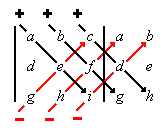
\includegraphics[scale=0.6]{sarrus}\\

\textbf{arithmetic rules:}\\
$\det (A \cdot B) = \det (A) \cdot \det (B)$\\
$\det (A^{-1}) = \det (A)^{-1}$\\
$\det\left(rA\right) = r^n\det A\,\,$,  for all $A^{n\times n}$ and scalars $r$

\subsection{rank}
Let A be a matrix.\\
$\text{rank}(A) = \text{columnSpace}(A) = \text{rowSpace}(A)$ \\
\quad = number of linearly independent column vectors of A\\
\quad = number of non-zero rows in A after applying Gauss\\

\subsection{row space}
The row space of a matrix is the set of all possible linear combinations of its row vectors.\\
Let $A$ be a matrix and $R$ a row-echelon form of $A$.\\
Then the set of nonzero rows in $R$ is a basis for the row space of $A$.

\subsection{column space}
Let $A$ be a matrix and $R$ a row-echelon form of $A$.\\
A basis for the column space of $A$ can be obtained by taking the columns of $A$ that correspond to the columns with leading entries in $R$.

\subsection{kernel == nullspace}
$\text{kern}(A) = \left\{ x\in\mathbb{R}^n : Ax = 0 \right\}$ \quad (the set of vectors mapping to 0)\\

\sect{rank and nullity}
$rank(A) + nullity(A) = n$\\

\subsection{trace}
defined on n$\times$n square matrices: $\mathrm{tr}(A) = a_{11} + a_{22} + \dots + a_{nn}$\\
(sum of the elements on the main diagonal)


\subsection{span}
Let $v_1,\dots,v_r$ be the column vectors of A. Then:\\
The span of $A$ may be defined as the set of all finite linear combinations of elements of $A$.\\
$\operatorname{span}(A) =  \{ {\lambda _1 v_1  +  \dots  + \lambda _r v_r \mid \lambda _1 , \dots ,\lambda _r  \in \mathbb{R}} \}$

\subsection{properties}
\textbf{square}: $N \times N$\\
\textbf{symmetric}: $A = A^T$\\
\textbf{diagonal}: 0 except $a_{kk}$\\

\sect{orthogonal} $A^T = A^{-1}$
$\Rightarrow$ normal and diagonalizable\\

\sect{nonsingular}
$A^{n \times n}$ is nonsingular = invertible iff:\\
\begin{itemize}
\item There is a matrix $B := A^{-1}$ such that $AB = I = BA$\\
\item $det(A) \ne 0$\\
\item $Ax = b$ has exactly one solution for each $b$, $b = 0$ included\\
\item The reduced row-echelon form of $A$ is an identity matrix\\
\item $A$ can be expressed as a product of elementary matrices.\\
\item The column vectors of $A$ are linearly independent\\
\item The rows of $A$ form a basis for $\mathbb{R}^{n}$\\
\item The columns of $A$ form a basis for $\mathbb{R}^{n}$\\
\item $\text{rank}(A) = n$\\
\end{itemize}

\smallbreak
$\Rightarrow det(A^{-1}) = \frac{1}{det(A)}$\\
$\Rightarrow (A^{-1})^{-1} = A$\\
$\Rightarrow (A^{T})^{-1} = (A^{-1})^{T}$

\sect{block matrices}
Let B, C be submatrices, and A, D square submatrices. Then:\\
$\det\begin{pmatrix}A& 0\\ C& D\end{pmatrix} = \det\begin{pmatrix}A& B\\ 0& D\end{pmatrix} = \det(A) \det(D)$

\sect{permutation matrix}
Permutation matrix $P = R_{k} \dots R_{1}$.\\
Row swap matrices $R_{i}$ are symmetric and that they are their own inverses.\\
$P^{-1} = R_{1} \dots R_{k} = R_{1}^{T} \dots R_{k}^{T}$.\\
Thus $P^{-1} = P^{T}$.

\sect{transpose properties}
$(A^T)^T = A$\\
$(AB)^T = A^TB^T$\\
$det(A^T) = det(A)$\\
$(A^T)^{-1} = (A^{-1})^T$

\subsection{compute powers}
$A = BDB^{-1}$. $D$ is a diagonal matrix.\\
$A^{n} = BD^{n}B^{-1}$.\\
$\begin{bmatrix}0& 1\\ 1& 1\end{bmatrix} = B \begin{bmatrix}\phi_{+}& 0\\ 0& \phi_{-1}\end{bmatrix}B^{-1}$\\
$\phi_{+} = \frac{1 + \sqrt{5}}{2}$; $\phi_{-} = \frac{1 - \sqrt{5}}{2}$; $\phi_{+}\phi_{-} = -1$\\
$B = \begin{bmatrix}1& 1\\ \phi_{+}& \phi_{-}\end{bmatrix}$\\
$B^{-1} = \frac{1}{\phi_{+} - \phi_{-}} \begin{bmatrix}-\phi_{-}& 1\\ \phi_{+}& -1\end{bmatrix}$\\
$fib[n] = \frac{\phi_{+}^{n} - \phi_{-}^{n}}{\phi_{+} - \phi_{-}}$
$\begin{bmatrix}0& 1\\ 1& 1\end{bmatrix}^{n} = \frac{1}{\phi_{-} - \phi_{+}}\begin{bmatrix}\phi_{+}^{n-1} - \phi_{-}^{n-1}& \phi_{-}^{n} - \phi_{+}^{n}\\ \phi_{-}^{n} - \phi_{+}^{n}& -\phi_{+}^{n+1} + \phi_{-}^{n+1}\end{bmatrix}$

\subsection{Cramer’s Rule}
$Ax = b$\\
$x_{1} = \frac{det(A_{1 \leftarrow b})}{det(A)}$
$x_{2} = \frac{det(A_{2 \leftarrow b})}{det(A)}$
$x_{3} = \frac{det(A_{3 \leftarrow b})}{det(A)}$

\subsection{Cofactor}
Let $M_{ij}$ be the matrix $A$ with the $i^{th}$ row and $j^{th}$ column removed.\\
$C_{ij} = (-1)^{i+j}det(M_{ij})$\\
$det(A) = \sum_{j=1}^{n}(-1)^{i+j}a_{ij}det(M_{ij})$\\
$A^{-1} = \frac{C^{T}}{det(A)} \Rightarrow AC^{T} = det(A)I_{n}$

\subsection{Orthogonality}
Two vectors are orthogonal if and only if\\
$u^{T}v = 0$

\subsection{subset vs subspace}
A subset is just a set of elements from the vector space.\\
A subspace of a vector space is a subset that follow the 3 rules.

\sect{subspace}
The $\cap$ of two subspaces of $\mathbb{R}^{n}$ is still a subspace of $\mathbb{R}^{n}$.\\
The $\cup$ of two subspaces of $\mathbb{R}^{n}$ may not be a subspace of $\mathbb{R}^{n}$.

\subsection{dimension}
The dimension of a vector space $V$ , denoted by $dim(V)$, is defined to be the number of vectors in a basis for $V$.\\
In addition, we define the dimension of the zero space to be zero.

\sect{solving $[A|b]$}
Do Gaussian elimination on the augmented matrix $[A|b]$.\\
If $rank([A|b]) > rank(A) \Rightarrow Ax = b \text{ does not have a solution} \Rightarrow \text{b is not in the column space of } A$

\subsection{dimension general case}
Vector space $M(m, n)$ of all m-by-n matrices.\\
The dimension of this space is $m \times n$\\
Let $E_{ij}$ be the m-by-n matrix that is all zero except for a 1 in the $(i, j)$ entry.\\
The all the $E$ matrices are a basis for $M(m, n)$

\subsection{Reasoning about dimension}
Let $S \subseteq \mathbb{R}^{n}$ be a subspace:\\
\quad if vectors $v_{1}, \dots, v_{k} \in S$ are linearly independent, then\\
\quad \quad $dim(S) \geq k$\\
\quad if $span({v_{1}, \dots, v_{k}}) = S$ then\\
\quad \quad $dim(S) \leq k$

\subsection{General solution for $Ax = b$}
$x$ = (the general solution of $Ax = 0$)\\
\quad $+$ (one particular solution of $Ax = b$).\\
e.g\\
$x = s*v_{1} + t*v_{2} + a$\\ $v_{i}$ spans nullspace of $A$\\$a$ is a particular solution.
\end{multicols}
\end{document}


\end{document}
